%% Based on a TeXnicCenter-Template by Tino Weinkauf.
%%%%%%%%%%%%%%%%%%%%%%%%%%%%%%%%%%%%%%%%%%%%%%%%%%%%%%%%%%%%%

%%%%%%%%%%%%%%%%%%%%%%%%%%%%%%%%%%%%%%%%%%%%%%%%%%%%%%%%%%%%%
%% HEADER
%%%%%%%%%%%%%%%%%%%%%%%%%%%%%%%%%%%%%%%%%%%%%%%%%%%%%%%%%%%%%
\documentclass[a4paper,12pt]{report}
% Alternative Options:
%	Paper Size: a4paper / a5paper / b5paper / letterpaper / legalpaper / executivepaper
% Duplex: oneside / twoside
% Base Font Size: 10pt / 11pt / 12pt


%% Language %%%%%%%%%%%%%%%%%%%%%%%%%%%%%%%%%%%%%%%%%%%%%%%%%
\usepackage[USenglish]{babel} %francais, polish, spanish, ...
\usepackage[utf8x]{inputenc}
%\usepackage[ansinew]{inputenc}

\usepackage{lmodern} %Type1-font for non-english texts and characters


%% Packages for Graphics & Figures %%%%%%%%%%%%%%%%%%%%%%%%%%
\usepackage{graphicx} %%For loading graphic files
%\usepackage{subfig} %%Subfigures inside a figure
%\usepackage{pst-all} %%PSTricks - not useable with pdfLaTeX



%% Math Packages %%%%%%%%%%%%%%%%%%%%%%%%%%%%%%%%%%%%%%%%%%%%
\usepackage{amsmath}
\usepackage{amsthm}
\usepackage{amsfonts}


%% Other Packages %%%%%%%%%%%%%%%%%%%%%%%%%%%%%%%%%%%%%%%%%%%
%\usepackage{a4wide} %%Smaller margins = more text per page.
%\usepackage{fancyhdr} %%Fancy headings
%\usepackage{longtable} %%For tables, that exceed one page
\usepackage[dvipsnames]{xcolor}
\usepackage{subcaption}
\usepackage[export]{adjustbox}
\usepackage[a4paper, margin=2cm]{geometry}
\usepackage{float}
\usepackage{tikz,siunitx}	
\usepackage{xurl}
 \newenvironment{acknowledgements} {\renewcommand\abstractname{Acknowledgements}\begin{abstract}} {\end{abstract}} 
%%remove the paragraph indent for the whole document
\setlength\parindent{0pt}

\usepackage{listings}
%%%%%%%%%%%%%%%%%%%%%%%%%%%%%%%%%%%%%%%%%%%%%%%%%%%%%%%%%%%%%
%% DOCUMENT
%%%%%%%%%%%%%%%%%%%%%%%%%%%%%%%%%%%%%%%%%%%%%%%%%%%%%%%%%%%%%
\begin{document}

\pagestyle{empty} %No headings for the first pages.


%% Title Page %%%%%%%%%%%%%%%%%%%%%%%%%%%%%%%%%%%%%%%%%%%%%%%
%% ==> Write your text here or include other files.

%% The simple version:
%\title{Title of this document}
%\author{Firstname Lastname}
%%\date{} %%If commented, the current date is used.
%\maketitle

\begin{titlepage}

		\begin{figure}[t]

			\begin{subfigure}{0.5\textwidth}
			
\includegraphics[width=0.9\linewidth, left]{image/serval-logo-2-black.png}
			\end{subfigure}
		\end{figure}

    \begin{center}
        \vspace*{2cm}
				
        \Huge
        \textbf{\textcolor{BlueViolet}{Serval PROJECT}}
        
        \vspace{0.5cm}
        \LARGE
				\textcolor{blue}{Documentation for serval test network}
				\noindent\color{BlueViolet}\rule{\textwidth}{2pt}
		\end{center}        
		\vspace{1.5cm}
		
		\vfill
		
		\noindent\textcolor{Blue}{
		\large \noindent Author: Stephane IMBERT\\
		Exchange student at Flinders University\\
		Project supervisor: Dr Paul Gardner-Stephen
		}
		
		\vspace{2cm}	
		
		\noindent\large Submitted to the School of Computer Science, Engineering, and Mathematics in the Faculty 
of Science and Engineering in partial fulfilment of the requirements for the degree of Master of Computer Science at Flinders University –
 Adelaide Australia.
		
		\vspace{1.5cm}
		\noindent\large
		Flinders University at Tonsley\\
		1284 South Road\\
		Clovely Park SA 5042
\end{titlepage}

I certify that this work does not incorporate without acknowledgment any material previously 
submitted for a degree or diploma in any university; and that to the best of my
 knowledge 
and belief it does not contain any material previously published or written by another person 
except where due reference is made in the text.

\newpage

\begin{abstract}

The Serval project started 8 years ago with the goal of creating an affordable communication solution that will work when the classic mobile network is not working. The team working on this project realised that some places didn't have a communication tool and that communication network may fail because of natural disasters (earthquakes, ...) or human disasters (terrorist, network congestion). That's why they wanted to create a new communication solution.

After working for several years, they recently did some real testing in Vanuatu. These tests revealed some faults in their solution and the Mesh Extender in particular. The Mesh Extender, is an important device in the Serval network as it plays two roles:
\begin{itemize}
	\item It is an access point to the network for the phone thanks to its Wi-Fi interface
	\item It is a router in the network. All the Mesh Extenders connect to each other via Wi-Fi to create a mesh network.
\end{itemize}

In order to find new faults and fix known ones, the team needed a test network. They currently lack a real practical test network in the building of Tonsley. My project was to design and deploy a test network in two months. 
In this thesis, I will present the solution I have come up with and how to install it. 
The test network developed has the following properties:
\begin{itemize}
	\item Affordable
	\item Easy to use
	\item Easy to expand
	\item Practical
	\item Easy to reproduce elsewhere
\end{itemize} 

The solution is based on affordable components. Indeed, for my project I had a budget of around 300Aud\$ for any component I was not able to find in the laboratory.
Therefore, the network part is based on small Linux routers (Gl-AR150 and GL-AR750). They have the advantages of being small, affordable and you have a full control over the OS and the software.

The solution to supervise the Mesh Extenders is based around a TCP client-server system written in C. To make it easier to use, a shell-like interface with basic commands was developed.



\end{abstract}


\begin{acknowledgements}


I would like to express my gratitude to all the people who helped me during the project and made it a reality in the first place.

First, I would like to thank my supervisor, Paul Gardner-Stephen, for his precious help during the project, all the advices he gave me and for trusting me in this project. Thanks to him, I feel I have become a better engineer.

I would also like to thank Flinders for accepting me as an exchange to them. Thanks to them, I was able to come here in Australia and live one of the greatest experience of my life as a student.

Finally, I want to thank my home school, INSA, for giving me the possibility to study abroad.




\end{acknowledgements}


%% Inhaltsverzeichnis %%%%%%%%%%%%%%%%%%%%%%%%%%%%%%%%%%%%%%%
\tableofcontents %Table of contents
\cleardoublepage %The first chapter should start on an odd page.


\pagestyle{plain} %Now display headings: headings / fancy / ...

%% The List of Figures
\clearpage
\addcontentsline{toc}{chapter}{List of Figures}
\listoffigures




%%%%%%%%%%%%%%%%%%%%%%%%%%%%%%%%%%%%%%%%%%%%%%%%%%%%%%%%%%%%%
\chapter{INTRODUCTION}




\section{Communication matters}

We live in a world where we are almost always connected to internet. Most of the people are using a smartphone. They can connect their phones to a cellular network owned by an operator such as Vodafone, Telstra or Optus in Australia and go to internet, send text or call a close relation. We now live in a world where we can communicate with anyone on the planet at almost anytime.\\
Communication has become a need for us. Daily we are communicating with people far from us. It can be for our job. We might be working in a team spread across multiple cities or country. It can be with our family and friends. Whatever the case, communication is crucial. We want to be able to contact someone at anytime and anywhere.\\
There is one situation where communication matters the most: during disasters whether they are natural (earthquakes, storm, tsunami, …) or not (terrorist attack). During such events, emergency services need to be able to communicate. Indeed, to save people’s lives, they must work very efficiently. Thus, they need to communicate so they can organise their team work.\\
For all these reasons, we should be able to communicate at anytime and anywhere.





%%%%%%%%%%%%%%%%%%%%%%%%%%%%%%%%%%%%%%%%%%%%%%%%%%%
%								Next Section 											%
%%%%%%%%%%%%%%%%%%%%%%%%%%%%%%%%%%%%%%%%%%%%%%%%%%%

\section{Reality is different}

We would like to be able to call our family at anytime and everywhere in the world. However, it’s still not possible. To be able to call someone you currently need some sort of connection to a cellular network. But these networks don’t cover the whole land even in a country as developed as Australia. One of the three big Australian operator, Telstra, display a map showing their current coverage on their website

\begin{figure}[H]
	\centering
	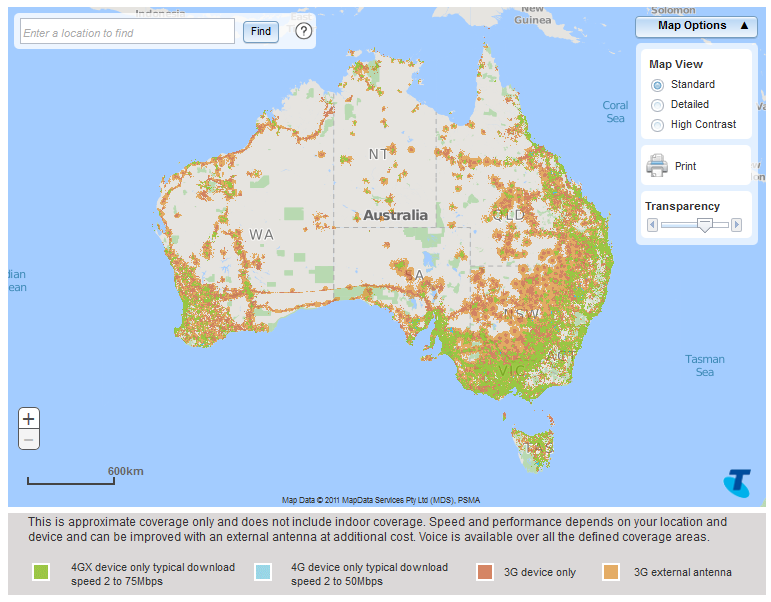
\includegraphics[width=0.6\textwidth]{image/Teslra-coverage.png}
	\caption{Telstra cellular coverage (Telstra.com.au, 2018)}
	\label{fig:Telstra}
\end{figure}

As we can see on the previous figure, Telstra cellular network is far from covering all Australia. Telstra network only covers places where people live. Telstra has no interest in places where no one live. Indeed, why would they extend their network in a part of Australia where no one live. They will just lose money: investment with no new customers at the end. 
Before extending its coverage, an operator mainly looks at two points: how much money will it cost and how many new customers will I get. If after studying these two points, they realise that they will never get back the money they invested, then they won’t spread their coverage. This means that small isolated towns may never have any connection with the rest of the world.
Right now, you cannot communicate anywhere. Unfortunately, even the covered zone cannot communicate all the time.
Indeed, in several cases, the network will go down. The few main reasons for a network to go down are the following:
\begin{itemize}
	\item Natural disasters (earthquake, storm, tsunami, ….).
	\item Human disasters (terrorist attacks).
	\item Network congestion
\end{itemize}
	
Looking at the past news, it is easy to find natural disasters where a huge part of the network went down. For instance, in august 2017, the tropical storm Harvey destroyed a huge part of the mobile network in Texas (Brodkin, 2017). First, this hurricane “has caused outages for more than 148,000 Internet, TV, and phone customers” leaving this people unable to make call. But, more importantly, this storm has damaged more than “17 emergency call centers”. During a hurricane, being able to call emergency centre can be a matter of life and death. When 17 call centres are disturbed by a storm, it means rescue teams might not be as effective as they can be. 

A good example of human disaster which had a tremendous impact for the emergency services is the bombing in London in 2005 (London.gov.uk, 2007). During this event, the carrier networks went down. Indeed, because of the bombs, a lot of people used their phones to call their families and close relations. This led to a network congestion. The network had reached his full capacity and couldn’t be used by the emergency staff. 

As we can see from the few examples above, we still cannot communicate at anytime and anywhere. These examples also demonstrate the importance of communication. In addition to be a need for us, it can also save lives. Therefore, we should try to find a way to provide a system of communication which is available all the time and everywhere.
This kind of communication services is the purpose of an existing project: the Serval project. 





%%%%%%%%%%%%%%%%%%%%%%%%%%%%%%%%%%%%%%%%%%%%%%%%%%%
%								Next Section 											%
%%%%%%%%%%%%%%%%%%%%%%%%%%%%%%%%%%%%%%%%%%%%%%%%%%%

\section{Presentation of the Serval Project}
\subsection{Purpose of the project}

The Serval Project started 8 years ago. What inspired Paul Gardner-Stephen and Romana Challans to launch this project is the Haiti earthquake that happened in 2010 (Encyclopedia Britannica, 2017) (Gardner-Stephen et al., 2013). During this event, most of the cellular networks went down. Without any communication means, the rescue team had a lot of trouble to organise which led to more casualties. Therefore, the goal of the Serval Project is to offer a way of communication when the common ones are dysfunctional or unavailable.

In other words, they want to create a communication system available everywhere and at anytime.

To reach that goal, the solution must be low-cost. Indeed, if one wants to install a system everywhere it should be easy and cheap to deploy.



%%%%%%%%%%%%%%%%%%%%%%%%% Next Subsection

\subsection{Structure of the project}

The Serval Project uses the following structure:

\begin{figure}[H]
	\centering
	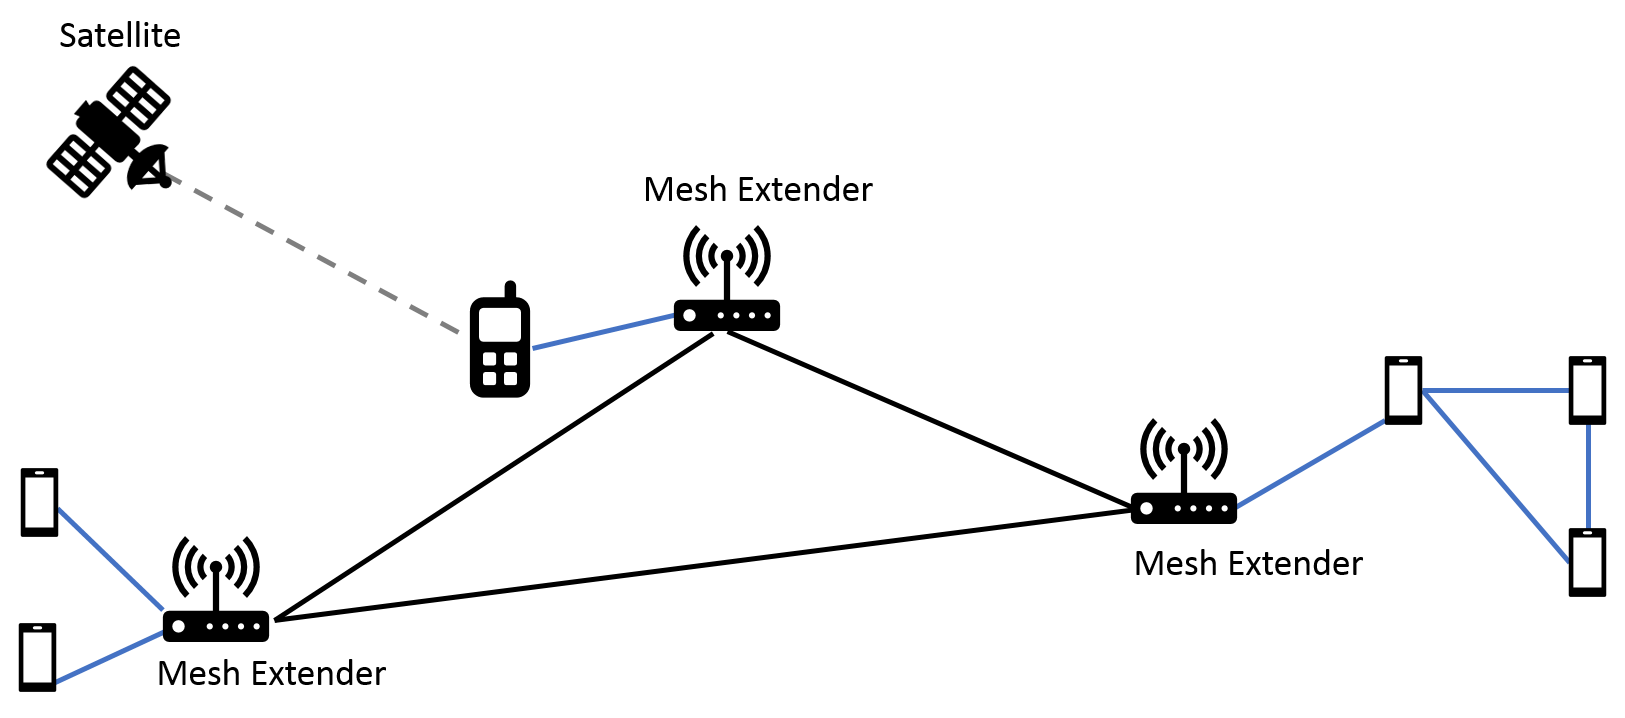
\includegraphics[width=0.6\textwidth]{image/Infra.png}
	\caption{Serval project structure}
	\label{fig:struct}
\end{figure}

\begin{tabular}{r@{: }l r@{: }l}
Legend & \\
\tikz[baseline]{\draw[ultra thick] (0,.5ex)--++(.5,0) ;}& UHF \\
\tikz[baseline]{\draw[ultra thick, color=blue] (0,.5ex)--++(.5,0) ;}& Wi-Fi\\
\tikz[baseline]{\draw[ultra thick, dashed] (0,.5ex)--++(.5,0) ;}& Satellite communication
\end{tabular}

As we can see on the previous picture, the Serval project uses a mesh network. A mesh network is a network where all the nodes are dynamically making connections with as many other nodes as possible. In the Serval project, the nodes are typically mobile phones, mesh extenders or devices for satellite connection.

This kind of structure has a few advantages. The connections are dynamically constructed which means that the network is easily scalable. Furthermore, since each device try to create as many links as possible, there are a lot of redundancy in the network. So even if a path between two devices breaks, there are still plenty other paths for the two phones to communicate.
The smartphones are using Wi-Fi to communicate which means that any person with a cellular can join the network by using an open-source, free application. 

However, Wi-Fi has a small range. In perfect conditions (free-space), Wi-Fi can reach around 200m. But in reality, in the best-case scenario, we can expect 80 to 100 m outdoor and 20 to 30m indoor. If the Wi-Fi was only used to interconnect the mobiles, the network wouldn’t reach very far. Thus, the mesh extenders were added. 
As their name suggest, the goal of the mesh extender is to extend the reach of the network. They are composed of 2 antennas:
\begin{itemize}
		\item A Wi-Fi antenna used for the communication between the user’s devices and the mesh extender
		\item A radio antenna, used between the mesh extenders
\end{itemize}


The radio transmission is designed to have a very long range (greater than 3km (Gardner-Stephen et al., 2013)). The mesh extenders play an important role in the project. They allow two users, who are very far from one and another, to communicate. Since they should be deployed at many places, they are designed to be low-cost and self-sufficient (for instance, solar panel can be used to power them). 

The last component of the structure is the satellite communication. This part is still not finished and is one of the upcoming project.

This structure allows the users to communicate by using an application (Serval Mesh).



%%%%%%%%%%%%%%%%%%%%%%%%%%%%%%%%%%%%%%%%%%%%%%%%%%%
%								Next Section 											%
%%%%%%%%%%%%%%%%%%%%%%%%%%%%%%%%%%%%%%%%%%%%%%%%%%%

\section{Statement of the problem}

Even though a lot of work has been done since 2010, the project is still not over yet. Therefore, there are still some faults, failures. 
Last year, there was a pilot deployment in Vanuatu. This pilot revealed some software and hardware faults and failures within the mesh extenders. These faults mean that in some cases, the mesh network doesn’t work and no communication is available. Therefore, the goal of the project (offering a system of communication when the usual ones fail) is not reached yet. 
In order to fix the found faults, you need to be able to recreate them. Currently, the team, here at Tonsley, lacks a real environment testbed to reproduce these faults and find new ones. Therefore, the goal of my project is to design a complete, practical test network for the Mesh Extenders and deploy it in Tonsley.

Through my project I will try to answer the following research questions:
\begin{itemize}
	\item How to design a test network for a Mesh Extender?
	\item What are the key points such testbed should answer?
	\item How can we be sure the testbed is not affecting the Mesh Extender normal functioning?
\end{itemize}

%%%%%%%%%%%%%%%%%%%%%%%%%%%%%%%%%%%%%%%%%%%%%%%%%%%%%%%%%%%%%


%%%%%%%%%%%%%%%%%%%%%%%%%%%%%%%%%%%%%%%%%%%%%%%%%%%%%%%%%%%%%
\chapter{Literature review}

\section{History of the Mesh Extender}

This project is based around the Serval Mesh Extender. The Serval Mesh Extender is a low-cost open-source infrastructure-independent telecommunications relay device (Gardner-Stephen et al., 2017a). In other word, it is a radio device capable to build a mesh network with other Mesh Extender. Through this network, it allows user to send messages. It is designed to be affordable and open-source.

The Serval project started 8 years ago. During this period, the Mesh Extender has been modified a lot of time and will be modified again.

At the beginning, the team was trying to enable Android smart-phones to communicate directly. The android phones will create self-organizing ad-hoc mobile telecommunications networks using Wi-Fi (Gardner-Stephen et al., 2017a). A few issues rose. First, the phone needed to be rooted. This is a modification that grant the user full control of the phone. This modification goes against the aim of the project. Indeed, the Serval project's aim is to replace the current mobile communication system  when it is not working. Therefore, the Serval project would be used by non-tech people. They don't know how to root a phone.
The second problem with this solution was the consumption. The battery life of the phone could drop to an hour (Gardner-Stephen et al., 2017).

To solve these issues, the Serval team decided to create a helper device that will create and take care of the network. The phone will only have to connect to this device. The Mesh Extender was born:

\begin{figure}[H]
\begin{center}
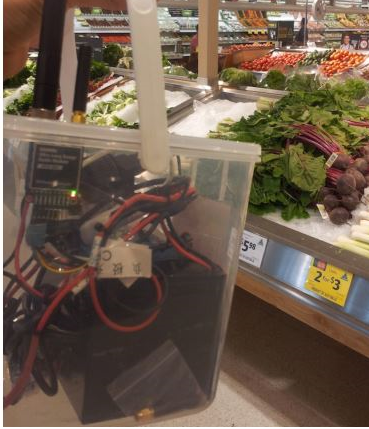
\includegraphics[width=0.3\textwidth]{image/meshextenderproto1.png}%
\caption{First prototype of the Mesh Extender (Gardner-Stephen et al., 2017a)}%
\label{figure:protoMesh}%-
\end{center}
\end{figure}


The Mesh Extender solved the two issues of the phone based solution and even bring a new advantage.
Since, they are creating, designing the Mesh Extender, they have a better control of the solution and less restriction. For instance, they were able to add other radio types such as a RFD900 (Gardner-Stephen et al., 2017a).



However, they quickly faced a major issue with this prototype. If you don't know it's a radio device, you may think it's a bomb. Hence, they add to work on the appearance of the Mesh Extender. Using 3-D printing, they created a new generation of the Mesh Extender:


\begin{figure}[H]
\begin{center}
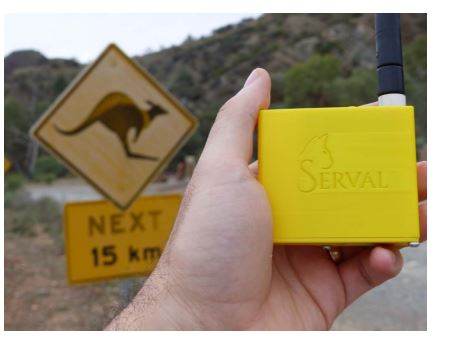
\includegraphics[width=0.4\textwidth]{image/meshextenderproto2.png}%
\caption{Seconde version of the Mesh Extender (Gardner-Stephen et al., 2017a)}%
\label{figure:protoMesh2}%-
\end{center}
\end{figure}


With this new generation, only the look changed. The component inside the Mesh Extender remained the same.
The last generation of the Mesh Extender changed that. It was design to have improved features and be ready for manufacture.


\begin{figure}[H]
\begin{center}
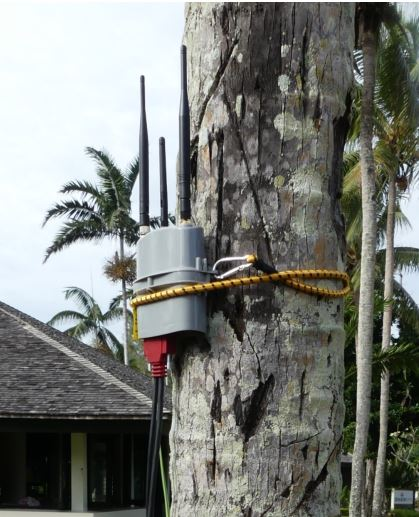
\includegraphics[width=0.4\textwidth]{image/meshextenderproto3.png}%
\caption{Latest version of the Mesh Extender in its natural environment (Gardner-Stephen et al., 2017a)}%
\label{figure:protoMesh3}%-
\end{center}
\end{figure}


The story of the Mesh Extender teaches us a lot for this project. First, the Mesh Extender is a product created years ago and that keeps evolving. When creating the test network, we have to think of the current features but also keep in mind that it may evolve or change in the future. 
The design of the Mesh Extender also gives us information on the philosophy behind the project. The team has a strong will to create affordable solutions using free open-software. The test network should reflect that philosophy.




\section{Pilot in Vanuatu}

Last year, the Serval team went to Vanuatu. A few conclusions were drawn from this trip. First, there is a strong need in Pacific nations for communication system such as the one proposed by the Serval project (Gardner-Stephen, 2017b). The Serval project is really interesting for Pacific nations like Vanuatu. First, since it is using solar power, it is self-sufficient. Second, the look of the product is rather professional. Finally, the Serval team is not a commercial for-profit operation(Gardner-Stephen, 2017b). 

Another goal of the trip in Vanuatu was to prove that the Serval Mesh Extender can work in a tropical-maritime environment (Gardner-Stephen, 2017b).

Finally, the last objective was to test the technology and find faults (Gardner-Stephen, 2018b).

Overall, the trip was a success. It proved that the Serval Mesh technology is working. But some faults were found and need to be fixed. All the data collected during the tests in Vanuatu will be very helpful to fix these faults. But in the long term, the team realised it will be beneficial to have a test network here at Tonsley. It could be used to understand the known faults and fix them but also to discover new ones.






\section{The current test network}
\subsection{Description of the test bed}


During the beginning of April, Paul installed an indoor test network at Tonsley.
The initial goal of this set-up was to verify if some bugs have been fixed. 

In the building, 13 points are linked to the Telecommunications Lab through copper and fibre. Therefore, we can easily place some Mesh Extenders at different location in the building. That's what Paul has done. 
At 4 different sites in the building, Paul installed one Mesh Extender. Hence, he created a multi-hop UHF network.

The repartition of the Mesh Extenders is the following:
\begin{itemize}
	\item 1 on the first floor
	\item 2 on the fourth floor
		\subitem 1 in the Telecommunications Lab
		\subitem 1 at the opposite side of the floor
	\item 1 on the fifth floor	
\end{itemize}
	

\begin{figure}[H]
	\centering
	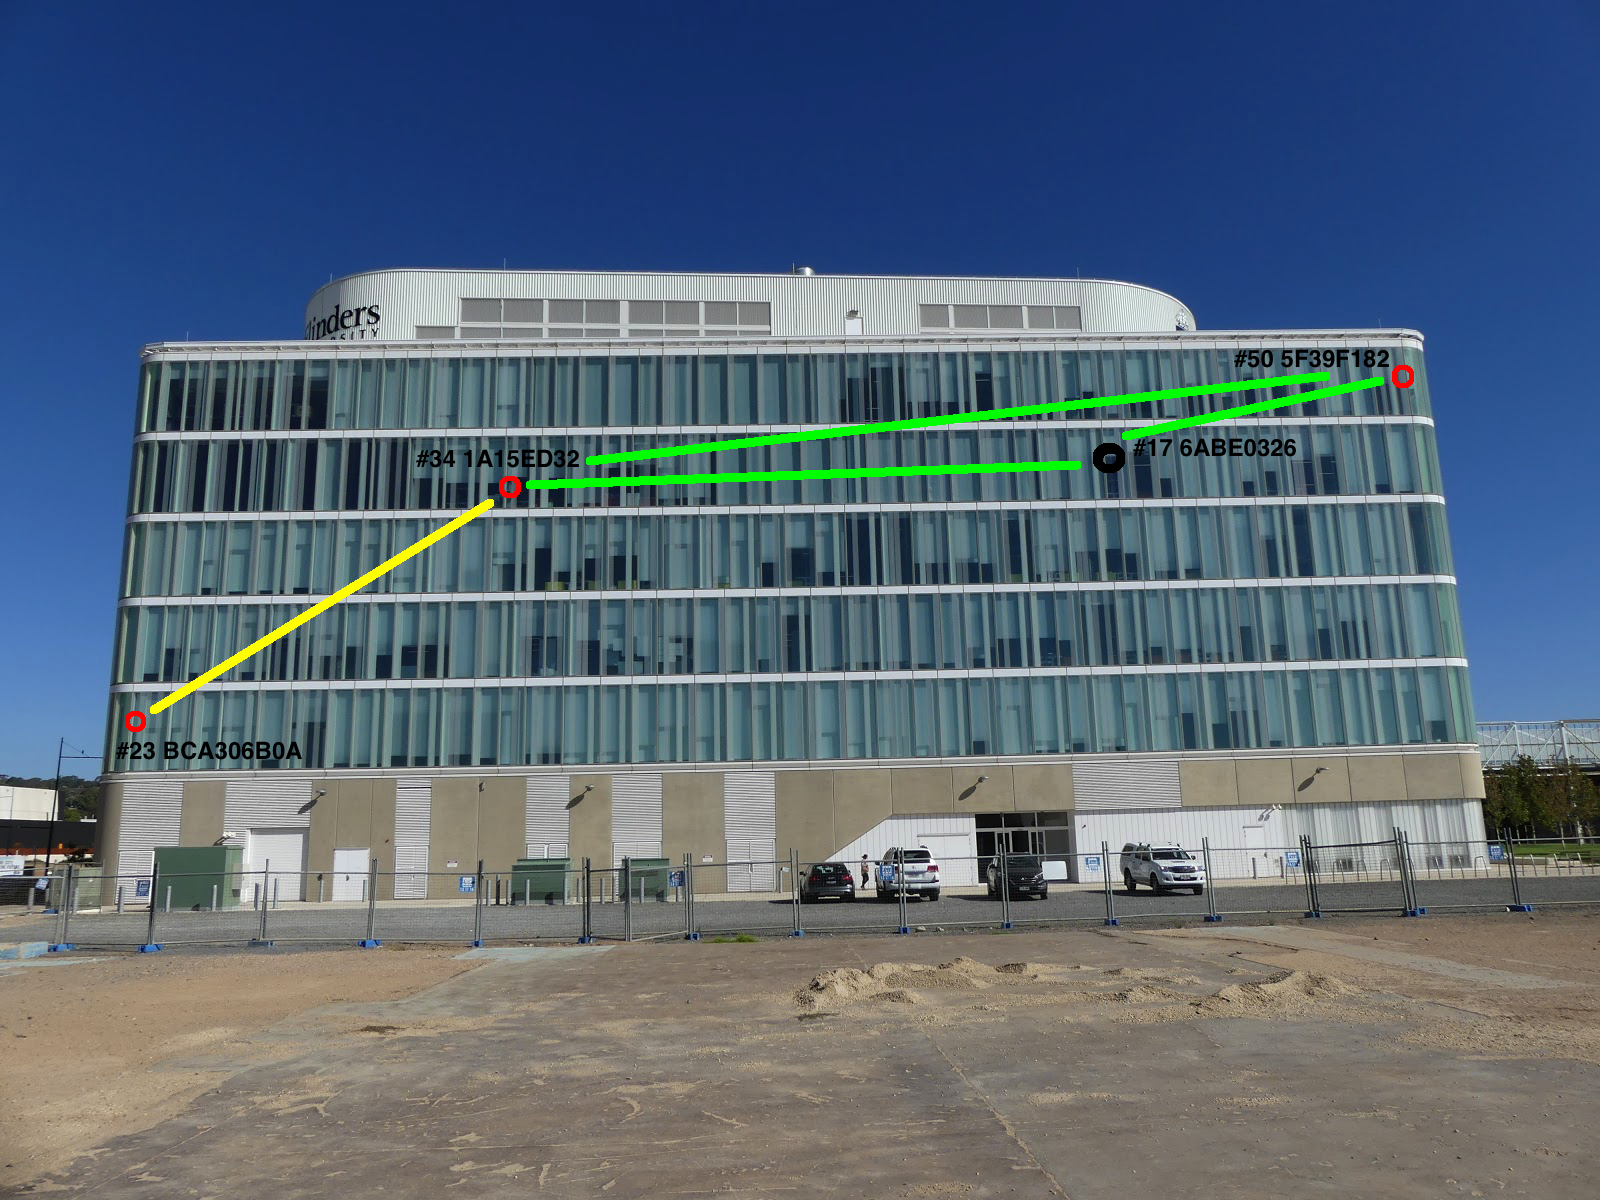
\includegraphics[width=0.6\textwidth]{image/TonsleyMeshExtenderLocations.png}
	\caption{Mesh Extender location (Gardner-Stephen, 2018a)}
	\label{fig:figure3}
\end{figure}


Since this network is supposed to be a multi-hop UHF, network, we want the Mesh Extenders to connect to each other using UHF and not Wi-Fi. For most of them, it is not a problem. Indeed, the Mesh Extenders are far enough from each other or the signal is heavily reduced by obstacles (walls for instance) for them to be able to connect with Wi-Fi.
However, the Mesh Extender on the fifth floor and one of the Mesh Extender on the fourth floor were able to communicate using Wi-Fi. Therefore, the Wi-Fi antenna was removed for one of the Mesh Extender(\#34 on the above picture).

With this set-up, we have a basic but functioning UHF network. We can use it to test some faults and fixes.


\subsection{Limitations of the current test network}

As explained previously, the current test network is made of 4 Mesh Extenders scattered across the building. This network is very basic and hence quick to install. However, it has some strong shortcomings.

The main issue with this network is its inconvenience. Indeed, this is just a UHF network, it doesn’t use Wi-Fi at all. Therefore, to test the network, you have to set-up a mobile at one of the site. Then move to another site and use a second phone to send a message to the first one. At the same time, you need to use computers to manually supervise each UHF link and each Wi-Fi connection involved in the communication. It can obviously be done but it will quickly become an hindrance to use repeatedly.

The second problem is the diversity. Since we only have Mesh Extenders on each site, we can only do basic test. If we want to do more complex tests, we need to go on each site to modify the set-up.

The last big problem is the current of short term improvement. Since the network is very basic, you cannot easily improve it. You cannot quickly add new features. You will need to add devices and heavily modify it to do so.



%%%%%%%%%%%%%%%%%%%%%%%%%%%%%%%%%%%%%%%%%%%%%%%%%%%
%								Next Section 											%
%%%%%%%%%%%%%%%%%%%%%%%%%%%%%%%%%%%%%%%%%%%%%%%%%%%

%%%%%%%%%%%%%%%%%%%%%%%%%%%%%%%%%%%%%%%%%%%%%%%%%%%%%%%%%%%%%


%%%%%%%%%%%%%%%%%%%%%%%%%%%%%%%%%%%%%%%%%%%%%%%%%%%%%%%%%%%%%











%%%%%%%%%%%%%%%%%%%%%%%%%%%%%%%%%%%%%%%%%%%%%%%%%%%%%%%%%%%%%


%%%%%%%%%%%-%%%%%%%%%%%%%%%%%%%%%%%%%%%%%%%%%%%%%%%%%%%%%%%%%%
\chapter{Presentation of the new test network}




\section{Goals for the new testbed}


The main goals for the new testbed are the following:
\begin{itemize}
	\item A test network as close as possible to a real life situation
	\item Possibility to remotely supervise both the Wi-Fi and UHF (Ultra High Frequency) communications
	\item Easy to use
	\item	Easy to reproduce elsewhere
	\item Affordable
	\item Easy to expand
\end{itemize}

This is a list of the features I was aiming for in this project. 
The network should be as close as possible to a real life situation. Indeed, if we want to test the Mesh Extenders, it is better to test them in a coherent scenario. We want them to be far enough from each other, so they don't rely only on Wi-Fi. We want them to be connected to other devices who can use the Serval network (phones for example). Obviously we will never have a true real situation since we are locked in the building and cannot set-up the network outside of the building. We are also limited in the number of devices at our disposal. These two points are limitation we have to work with.

We want the network to be practical. In the current testbed, we have to move around the build between the sites to test it. In the new testbed, we should be able to test everything from the lab.

The new test network should be easy to use and reproduce. The team in the Lab are obviously expert on the Serval project and could work with a very particular test network. However, this network could be reproduced by other teams who want to work on the project. They may not be too familiar with the project at the beginning, but they will probably still want to use the test network. That's why it should be easy to use (should be user friendly and be well documented) and easy to reproduce (thanks to a good documentation). 

We want the test network to be affordable. The first reason for this is linked to the previous point. Indeed, if we want other people to be able to recreate the test network, it should be as least expensive as possible. Indeed, they may not have access to a lot of funds or may not want to spend too much money (they could work on the project as a tech enthusiast).
The second reason is the budget of the team. 

Finally, the testbed should be easy to expand. The team is still working on the Serval project, improving it and adding new functionalities. Therefore, the testbed may have to evolve to test these new features. 

All these wanted properties and the environment we are working with create constraints and challenges we have to deal with or overcome.


%%%%%%%%%%%%%%%%%%%%%%%%%%%%%%%%%%%%%%%%%%%%%%%%%%%
%								Next Section 											%
%%%%%%%%%%%%%%%%%%%%%%%%%%%%%%%%%%%%%%%%%%%%%%%%%%%

\section{Constraints and challenges}


There are a lot of constraints we need to work with.

The first constraint is the environment we are working with. Indeed, Mesh Extenders are designed to be far from each other. But here, we are setting up a test network inside a building. That means we need to check how the Mesh Extenders are connecting to each other. We want to make sure they are using UHF to connect to other Mesh Extenders. It will limit the number of Mesh Extenders we can use in the test network. Right now, we want to use only 4 Mesh Extenders, so it is still manageable.

The Mesh Extenders being close create another issue. We would like to be able to test them when the signal is low to see how they handle package errors. "Thankfully", the walls in the building are quite good at blocking radio signal. Therefore, with the basic set-up Paul noticed that the UHF signal between the Mesh Extender on the first floor and one Mesh Extender on the fourth floor was very low. He even had to put a better antenna to the Mesh Extender on the first floor to improve the signal.

The last constraint is time. The available time for the project is very short. Indeed, the project was started after the mid semester break at the end of April/ beginning of May. Therefore, I had two months to make it.

Constraints are imposed by your environment, your possibilities whereas challenges are imposed by yourself. For this project, the properties of the test network are creating many challenges.

First our budget is limited. We want an affordable solution. Therefore, we decided to limit the budget for this project to the amount given by Flinders for the master project. It means that we have around 300 dollars to buy the needed device. Thankfully some of them were already in the Lab (the Mesh Extenders, cables, and the RFD900+). This budget means we don't have access to every solutions possible. Therefore, I had to work with limited devices and find work around.



Keeping in mind all these constraints and challenges, I came up with a design for the test network. 




%%%%%%%%%%%%%%%%%%%%%%%%%%%%%%%%%%%%%%%%%%%%%%%%%%%
%								Next Section 											%
%%%%%%%%%%%%%%%%%%%%%%%%%%%%%%%%%%%%%%%%%%%%%%%%%%%



\section{Design of the new testbed}


For the new test network, we will still have 4 sites at different places in the building. However, on each site, there will be more than just a Mesh Extender.

On each site we will find:
\begin{itemize}
	\item a Mesh Extender
	\item a small linux router
	\item an android phone
	\item a usb hub
	\item a RFD900+
\end{itemize}


In addition to this 4 sites, we add an additional set-up in the Telecommunication Lab. It will be the access point to the test network.

\subsection{Hardware used for the testbed}

First, for this test network, we will obviously need Mesh Extenders:
\begin{figure}[H]
\begin{center}
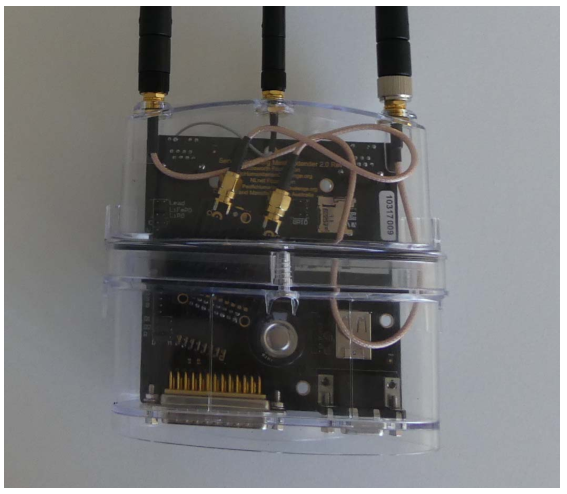
\includegraphics[width=8cm]{image/meshextender.png}%
\caption{Mesh Extender}%
\label{figure:ME}%-
\end{center}
\end{figure}


In this project we are also using small Linux routers to built the network we will use to supervise the Mesh Extenders.

The small routers we have chose to use are: the GL-AR150 and GL-AR750.

\begin{figure}[H]
\centering
\begin{subfigure}{.5\textwidth}
  \centering
	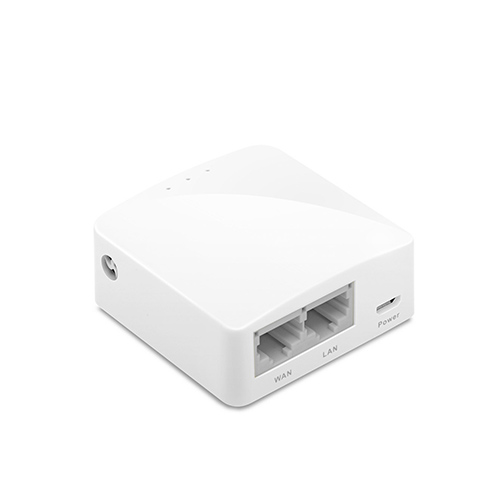
\includegraphics[width=8cm]{image/AR150.jpg}%
	\caption{GL-AR150}%
	\label{figure:AR150}%-
\end{subfigure}%
\begin{subfigure}{.5\textwidth}
  \centering
  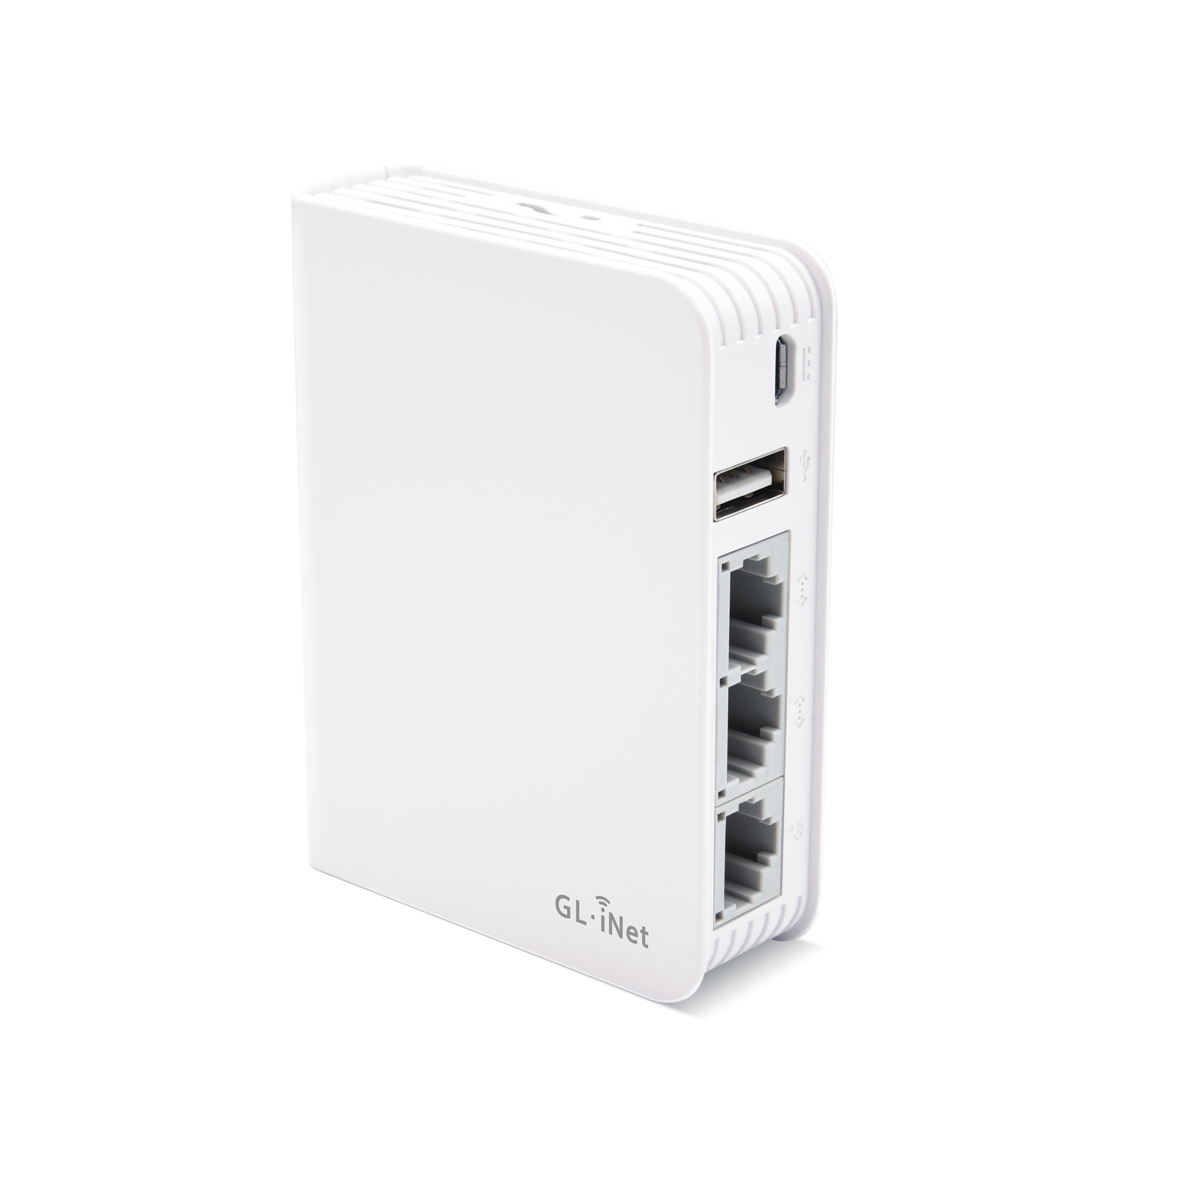
\includegraphics[width=8cm]{image/AR750.jpg}%
	\caption{GL-AR750}%
	\label{figure:AR750}%-
\end{subfigure}
\caption{Routers used for the testbed (source: https://www.gl-inet.com/)}
\label{fig:routers}
\end{figure}


These two routers are great for the test network. Indeed, they are small, affordable and we have a lot of freedom since their OS is based on a Linux kernel (the OS used for the Mesh extenders can also be put inside these routers).
The only issue we can have is the fact they do not have a lot of USB ports and no UHF radio. Therefore we need other devices:
\begin{figure}[H]
\centering
\begin{subfigure}{.5\textwidth}
  \centering
	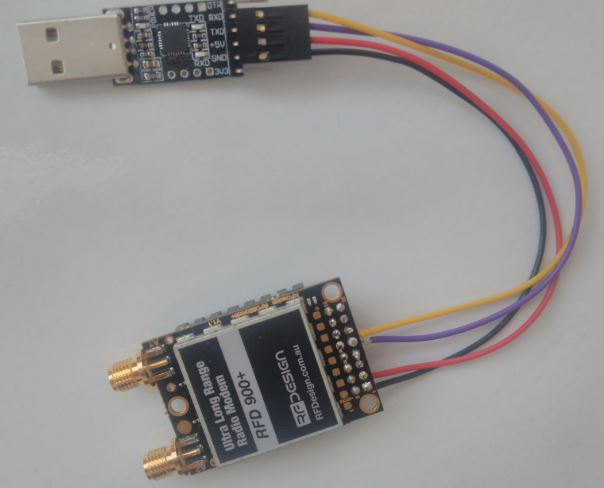
\includegraphics[width=8cm]{image/rfd900.jpg}%
	\caption{RFD900 with a serial to USB adapter}%
	\label{figure:RFD900}%-
\end{subfigure}%
\begin{subfigure}{.5\textwidth}
  \centering
  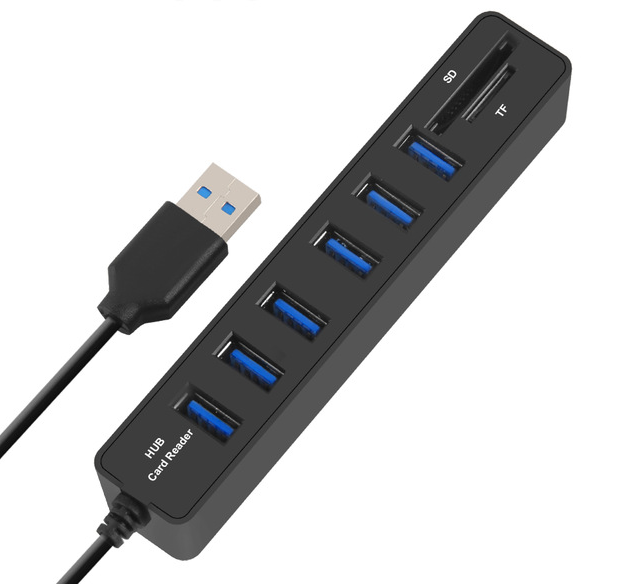
\includegraphics[width=8cm]{image/usbhub.jpg}%
	\caption{USB hub}%
	\label{figure:UsbHub}%-
\end{subfigure}
\caption{Other devices needed}
\label{fig:devices}
\end{figure}

To monitor the UHF packets of the Mesh Extenders, we need a RFD900+. Since the RFD900+ has a serial interface (pins), we need to create an adapter to plug it using USB.
We are using a USB hub to increase the number of USB ports on the router.

We now have all the needed hardware.





\subsection{Big picture}

As explained previously, there are two types of site in this test network:
\begin{itemize}
	\item The remotes sites where the Mesh Extenders are
	\item The main site used to interconnect the remotes sites and act as an access point
\end{itemize}

%figure main site








%figure remote site


\subsubsection{Global design of the network}

To interconnect them, we need to design a network solution.
I have come up with the following solution:
\begin{figure}[H]
\begin{center}
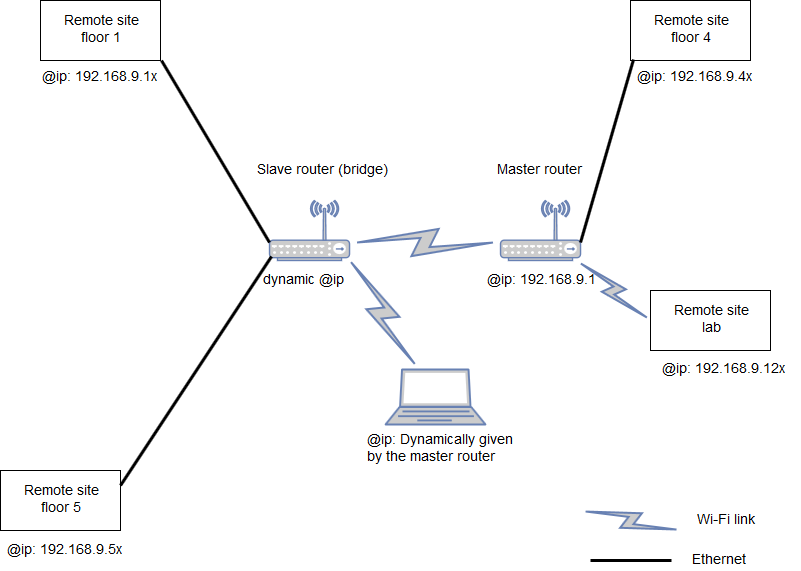
\includegraphics[width=\textwidth]{image/networkBigpicture.png}%
\caption{Big picture of the network}%
\label{figure:NetworkBigPicture}%-
\end{center}
\end{figure}

Since we want to be able to communicate with all the devices from the laboratory, the easiest solution is to create only one network. All the devices are in the same network and no routing is needed. The main router is an access point to the network and every communication has to go through it. Therefore, we have one point where we can control the network. These properties are very important. Indeed, since they are all in the same network, each device should be able to communicate with another through this network. It means that a Mesh Extender could use this network to send a message to another Mesh Extender using this network. However, since all communications have to go through the main router, we can avoid this situation. Indeed, we can set rules in the main router to prohibit communication between remote sites.

Another important point of this design is the distribution of IP addresses. The slave router and all the computers connected to this network will receive dynamic IP addresses. However, the remote sites will have fixed addresses for three reasons:
\begin{itemize}
	\item First, the remote servers need fixed hostnames for my software solution. By giving fixed IP addresses, the main router can also assign them a hostname
	\item The second reason is linked to the issue explained earlier. If they have fixed addresses, it will be easier to add traffic rules for these devices
	\item Finally it is easier to recognise each remote device is if they have fixed addresses.
\end{itemize}

In this design, the slave router is simply a bridge that extends the main router. GL-AR750 can be configured as bridges but only if they are linked with Ethernet. However, in my design, they are communicating by Wi-Fi. Luckily, we can simulate this bridge behaviour using a Linux packet called relayd.




\subsubsection{Global design of the software}

In this project, we are going to use C programs to remotely supervise the Mesh Extenders.
C language was chosen because:
\begin{itemize}
	\item It is a light and efficient language (which is great since our routers don't have a lot of power or memory)
	\item In the Serval project most of the coding was made in C. We can easily integrate other parts of the Serval project inside the test network.
\end{itemize}


I have decide to create a TCP client-server system composed of 3 files:
\begin{itemize}
	\item server.c which will be on the small routers
	\item client\_shell.c and client.c which will be for the user
\end{itemize}

I will explain what each file does in the next section.


A TCP client-server was not the only solution. However, I still opted for it because:
\begin{itemize}
	\item I was more used to code a TCP server and client than other solutions. Therefore, I will be faster using this solution.
	\item The libraries for TCP are quite old and should work on most devices.
\end{itemize}


The software part corresponds to the communication between a few programs:
\begin{itemize}
	\item The client\_shell and the client
	\item The client and the server
	\item The server and the RFD900+
\end{itemize}

For the communication between the server and the RFD900+, we use the driver in C developed by Paul. This part use the code of the LBARD git repository.

\hfill \break

We want to establish the following communication process:
\begin{figure}[H]
\begin{center}
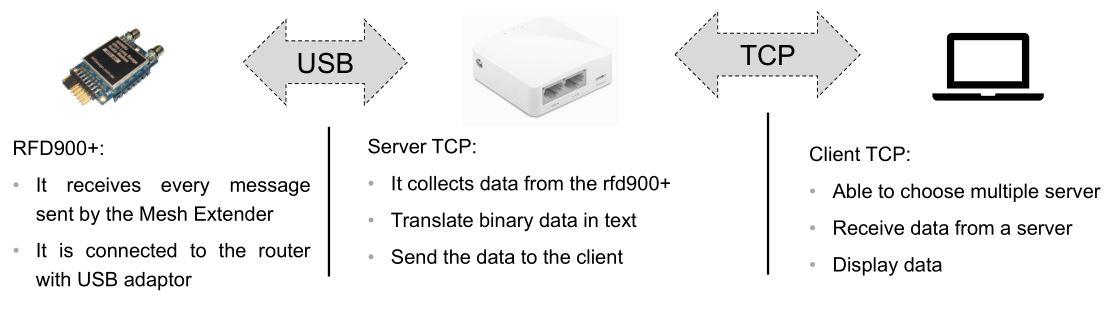
\includegraphics[width=\textwidth]{image/GlobalUHF.jpg}%
\caption{Mesh Extender's messages through the testbed}%
\label{figure:UHFmesh}%-
\end{center}
\end{figure}

\hfill \break



\hfill \break \underline{\large{\textbf{Communication between the server and the client}}}

The communication between the client and the server is very basic. Most of the time the client is only receiving packets from the server and displaying them on the computer.

But the client can also send a few messages to the server. These messages allow the client to close the communication with the server. Later they will also allow the client to change what is supervised.

\begin{figure}[H]
\begin{center}
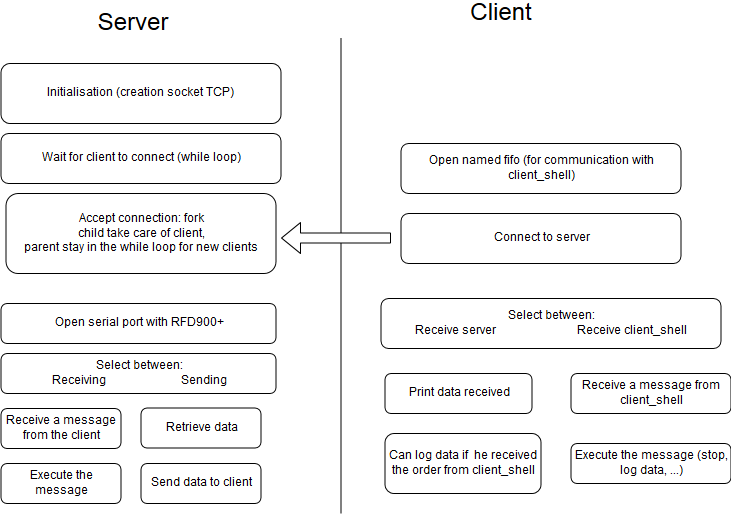
\includegraphics[width=\textwidth]{image/clientServer.png}%
\caption{Client and server communication}%
\label{figure:CS}%-
\end{center}
\end{figure}

The server start as a classic TCP server. It will create the socket for the server (a socket is basically the combination of source and destination IP address and port). Then it will listen on the socket to see if a client is trying to connect. Each time the server receive the connection, he starts a process to handle the client and keeps listening for new client. The process that handles the client work in a loop. In the loop, the process start by looking if the client sent a message. If he received a message from the client, the server analyses the message and execute the corresponding code. The messages can be used to stop the connection or change the behaviour of the server (what we want to supervise for instance). If the process does not receive a message from the client, it will send data to the client. By default, the data are the UHF packets sent by the Mesh Extenders.


\hfill \break \underline{\large{\textbf{Interactions between the client\_shell and the client}}}

The client\_shell is a shell-like interface that gives access to all the available functionalities.
It can:
\begin{itemize}
	\item Find the available servers using a file containing the hostnames of servers
	\item Launch a client
	\item Communicate with the client to send different orders such as
		\subitem "`STOP"' to close the connection
		\subitem "`LOG Filename"' to start logging the data
  \item Keep a list of all the current clients created
	\end{itemize}




\begin{figure}[H]
\begin{center}
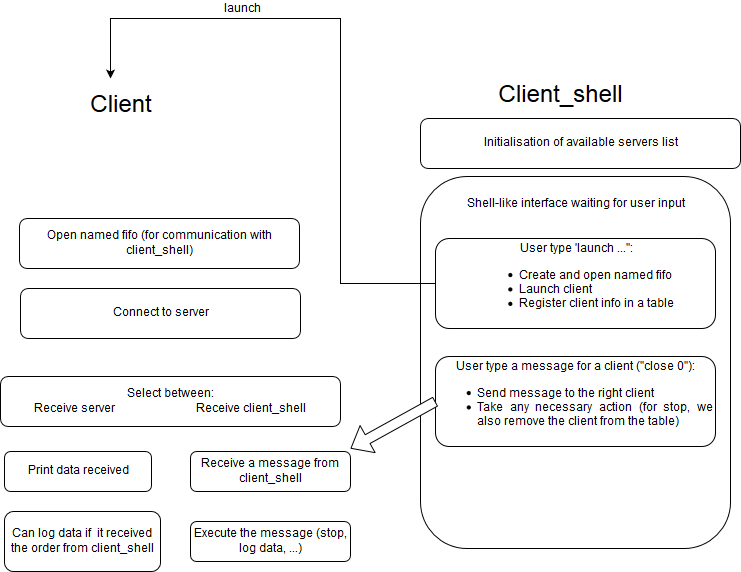
\includegraphics[width=\textwidth]{image/clientshellClient.png}%
\caption{Client and Client\_shell interaction}%
\label{figure:CSC}%-
\end{center}
\end{figure}



The client\_shell is a shell-like interface. It will start by initialising the list of server available. Using a file containing all the possible servers’ name, it will try to find which servers on the list is available at the moment. Then, it will wait for an input of the user.
The available commands are:
\begin{itemize}
	\item help: list the available built in functions
	\item exit: close the client\_shell
	\item launch: launch a client
	\item findServers: update the list of available servers
	\item displayServers: display the available servers
	\item close: close a client
	\item list: list the clients currently running 
	\item log: start or stop logging the data for one client
\end{itemize}

If you type a function but do not put the right parameters, the shell will display a short message
explaining how to use the function properly.


The client starts by opening the named FIFO (First In First Out: a pile of messages where they are read and written in the same order) that was created by the client\_shell. The client will receive order of the user through this named FIFO. Then the client will connect to the server. Once connected it will see if he received a message from the server or the client\_shell.
If he receives a message from the server, it will display it, and he can logged it if the user wants to.
If he receives a message from the client\_shell, it will understand the order and execute it. The order can be to log the data received from the server in a file or to close the connection with the server for example.

The client can be manually started by a user. In this case, the client will read the input from the client using the standard input. If the user type "STOP" in the shell where he started the client, it will close the connection with the server. Using the client this way is harder because you need to know exactly what to type to send an order to the client, and the client is constantly displaying text on the screen making it hard to type.



%%%%%%%%%%%%%%%%%%%%%%%%%%%%%%%%%%%%%%%%%%%%%%%%%%%%%%%%%%%%%


%%%%%%%%%%%%%%%%%%%%%%%%%%%%%%%%%%%%%%%%%%%%%%%%%%%%%%%%%%%%%
\chapter{Development of the new test network}


\section{Network installation}

For the network, I used GL-AR750 for the main site and GL-AR150 for the remote sites. There are not much work to do on the remote site. We just want to disable the DHCP on the LAN interfaces (because it will get an IP address and not distribute them).

For the two GL-AR750, we have a bit more work to do. We have two different routers to configure:
\begin{itemize}
	\item The master router who will distribute the IP addresses and control the network
	\item The slave router who will extend the master router's network and act as a bridge
\end{itemize}

\subsection{Master router configuration}

For the master router, we need to configure:
\begin{itemize}
	\item The LAN network (Wi-Fi and ethernet)
	\item The fixed addresses
\end{itemize}


We create a Wi-Fi network. It will be easier to use. Indeed, you don't need any cable and can connect your computer to the network wireless. We use fixed IP addresses and names for the remote routers. If they have fixed names, they will be easier to find for our client.


\subsection{Slave router configuration}

For the slave router, we need to configure the bridge function. The problem is that the GL-AR750 can not by default make a bridge between two Wi-Fi interfaces. He can bridge a Wi-Fi interface with an ethernet one or bridge two ehternet interfaces but not two Wi-Fi interfaces. Thankfully, a workaround exists. Indeed, there is package called relayd. This package lets you simulate a bridge behaviour. In fact, this package will transform our router into an invisible bridge. The devices that connect to the slave router, it will be like they are connected to the master router.


\begin{figure}[H]
\begin{center}
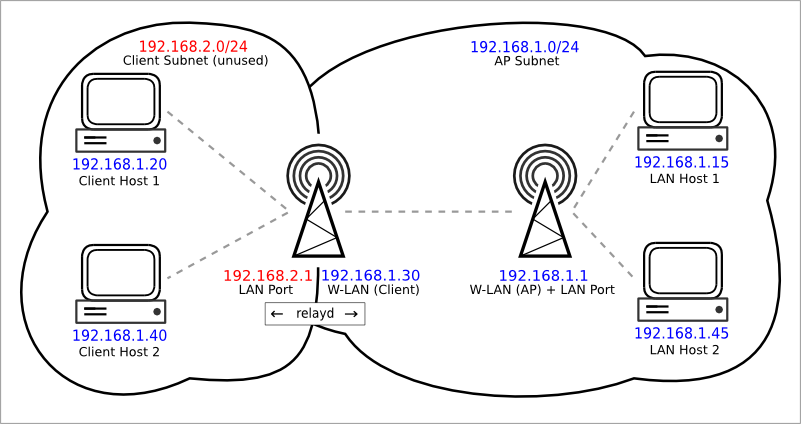
\includegraphics[width=0.7\textwidth]{image/802-11-routed-relay.png}%
\caption{Bridge network with relayd (source: https://wiki.openwrt.org/doc/recipes/relayclient)}%
\label{figure:relayd}%-
\end{center}
\end{figure}

We have two networks, one in blue and one in red. The master router is the one on the right (192.168.1.1). He is controlling the blue network. The slave router is connected to the master router. It is controlling the red network. We need to create this network for relayd but it is not really used. As you can see on the figure, the devices connected to the slave router are using addresses belonging to the blue network. For them, the slave router is just a bridge and does not really exist.





\section{Development of the server}

The server is a TCP server coded in C. It uses the LBARD code made by the Serval team. In particular, we are interested in one driver in the LBARD code. Indeed, the server needs to communicate with the RFD900+. 

\subsection{Building a TCP server}
The first thing I developed was the  TCP infrastructure of the server.
The infrastructure of the server is the following:
\begin{itemize}
	\item We first transform the server into a daemon (a daemon is process running in the background. It is not linked to a terminal and it can't print any data on the screen)
	\item We initialise the TCP socket
	\item We bind the socket
	\item We start listening on the socket to see incoming clients
	\item We have a while loop to accept any client
\end{itemize}

The while loop is where we handle the incoming client. In this loop the server wait for a client.
When receiving a client, the server will create another process (a child).
The main process will stay in the while loop to accept other client.
The child will exit the while loop and start communicating with the client. A communication in TCP is very basic.
You can either send data or receive data but you cannot do both at the same time. One thing to be aware is if the server tries to receive a message using the c function called "recv", he will be stuck until it actually receives a message.
So we need to make a choice. To do that, we can use the function called "poll". This function lets you analyse many sockets to see if one of them has received something. You precise a timer during which the function will look at the sockets. If a message is received on a socket, the poll function will end and tell you which socket has received a message. In this case, the child process will receive the message, understand it, and execute the correct part of the code. For instance, if it receives a "STOP" message, the child process will stop the communication and end.

If no message is received, the timer of the poll function will run out. In this case, the child process will send data to the client.

By default, the data sent are the UHF messages of the Mesh Extender.



\subsection{Integrating the LBARD code}

We want to send UHF messages. But, by default, the GL-AR150 does not have a radio interface able to perceive them. That's why we are using a RFD900+. To use it, we need to understand it using a driver. Paul developed a C driver for the RFD900+. Furthermore, the LBARD code is using this driver and is able to understand the RFD900+. So for my server, I reused the LBARD code made by the Serval team. Using all the needed files, I adapted them for the server.

I earlier explained that the first step of the server is to transform itself into a daemon. A daemon can not print data to the screen because it is not linked to any terminal and it doesn't have any standard output. However, the LBARD code is printing a lot of data. We need to remove all these printing. Instead of printing, we want to send them on the network to the client.
We have two solutions for that:
\begin{itemize}
	\item solution 1: Modify each function of the LBARD code to replace all the printing functions by using the function called "send". 
	\item solution 2: Redirect the standard output to the socket. It will mean that every function trying to print data will instead send them to the client  
\end{itemize}

The first solution is cleaner but very time consuming. The second solution is easier, faster and if someone want to add code to the server, he can do that without having to worry about the TCO aspect.

I actually implemented both solution. I modified a lot of the LBARD functions so they don't print data but rather send them. And as a backup for any mistake I could make and for the future users, I redirected the standard output to the network socket.




\section{Development of the client}

The client part is made of two programs: the client and the client\_shell.

\subsection{Development of the client}
The client is a basic TCP client that can also receive orders from the client\_shell.

First, need to prepare the client to receive orders from the client\_shell.
Since both programs are on the same computer, we can use named FIFO. A FIFO is a pile where you can store data, and they will be read in the same order as they have been put in the FIFO.
The client will open the named FIFO. The named FIFO was created by the client\_shell.
If the client was launched by the client\_shell, he will know the name of the FIFO and opened it. If the client was manually launched by the user, it will have no FIFO and will use the standard input to receive orders.



We now need to develop a basic TCP client:
\begin{itemize}
	\item We start by creating the socket
	\item We connect to the server
\end{itemize}
 
We are now ready to receive and send messages. But, in the same way as the server, the client needs to choose one option. This time, it will have to choose between:
\begin{itemize}
	\item Receiving data from the server
	\item Receiving orders from the client\_shell or the user
\end{itemize} 

We can once again use the function "poll". This function can look at any file descriptor to see if there is something to read. Thankfully, on Linux, everything is a file. So both the socket, the standard input and the named FIFO have file descriptors.
So we do a poll over these files descriptors and see which one has received something.

If the named FIFO (or the standard input) have received something, the client will read the order and execute. Right now, there are two possible orders:
\begin{itemize}
	\item "STOP" to close the connection. In this case, the client will send a "STOP" to the server to inform him
	\item "LOG" to start or stop logging the data received from the server
\end{itemize}

If the client received a message from the server, he will read the data and print them. It will also log them if it has received the order.

If both sockets have a message to read, the client will prioritise the order from the client\_shell.


Finally, I have added one functionality to the client. If the user tries to stop it without using the "STOP" message, the client will detect it (try to detect it) and send a "STOP" message to the server before stopping.


\subsection{Development of the client\_shell}

The client\_shell is a shell-like interface. To developed that interface I used the following tutorial: \url{https://brennan.io/2015/01/16/write-a-shell-in-c/}.

It explains how to create a shell in c and how to add built in functions.

So in this shell, we have two types of function:
\begin{itemize}
	\item Built in functions: function I have created. They are directly linked to the functioning of the test network.
	\item Classic shell functions
\end{itemize}

The available built in functions are:
\begin{itemize}
	\item help: list the available built in functions
	\item exit: close the client\_shell
	\item launch: launch a client
	\item findServers: update the list of available servers
	\item displayServers: display the available servers
	\item close: close a client
	\item list: list the clients currently running 
	\item log: start or stop logging the data for one client
\end{itemize}

All these functions are made so anyone can use the test network. You don't need to know how it work. With these functions, you have an easy access to the test network.

Let's explain some of them.

\hfill \break \underline{\large{\textbf{findServers}}}

The client\_shell is using a file containing all the possible names of the servers. With this file, he will check which server is available (see if the device is running with a ping). He will add each available server to a list. This function is runned when the client\_shell start to create the list.


\hfill \break \underline{\large{\textbf{displayServers}}}

The client\_shell will print all the servers available (list created by the findServers function). A number is associated to each server. This number can be used by the user to choose a server. The user doesn't have to remember each server address.

\hfill \break \underline{\large{\textbf{launch}}}

launch is used to launch a client. The user needs to precise which server he wants the client to connect to. There are two ways the user can precise the server:
\begin{itemize}
	\item the address of the server
	\item the number precised by the displayServers function
\end{itemize}
When launching a client, the client\_shell will add this client to a list, create the named FIFO and start the client.

\hfill \break \underline{\large{\textbf{list}}}

The function list can be used by the user to see all the clients running. Each client will have a number associated. This number can be used by the user to communicate with the client.

\hfill \break \underline{\large{\textbf{close}}}

The close function can be used to close a client. It will send a "STOP" message to a client. There are two ways of using this function:
\begin{itemize}
	\item Use the number of the client (number found using list) to close this client in particular.
	\item Type "close all" to shutdown all the clients.
\end{itemize}

\hfill \break \underline{\large{\textbf{log}}}

The log function can be used to tell a client to start or stop logging data. Once again, we can use this function in two ways:
\begin{itemize}
	\item "log X filename" to tell the client with the number X to start logging data in a file called filename
	\item "log X stop" to tell the client X to stop logging data
\end{itemize}


\section{Development of the phone and Wi-Fi parts}

Our test network should also monitor the Wi-Fi and allow the user to remotely control the phone.
Right now this two features are still in development. There is a temporary solution for the Wi-Fi and a proof of concept for the mobile part.

\subsection{How to monitor the Wi-Fi remotely}

I wanted to integrate some c code for this part but I unfortunately didn't have the time to do it. Right now, we have to use a temporary solution with the package tcpdump and wireshark (a graphic network tool to analyse messages going through the network).

tcpdump is a Linux package that can be installed on the routers. This package allow an user to scan all the messages going through an interface. Therefore, using this command, we can analyse the Wi-Fi communication going around the router.
We can install this package on the remote router.

Then on the computer in the lab, you simply have to use the following command:

\begin{lstlisting}[language=bash]
ssh root@192.168.8.11 tcpdump -i wlan0 -U -s0 -w - 'not port 22' | ... 
... sudo wireshark -k -i -
\end{lstlisting}

With this command, we launch the command tcpdump on the remote router. It will analyse the Wi-Fi interface called wlan0. Then the result of the tcpdump command is sent to our computer and displayed through wireshark. 


\subsection{How to remotely control a phone}

I managed to remotely control a phone using virtual machines. I had the phone plugged into one virtual machine, and I was controlling the phone in the other virtual machine.

All the component used for this solution were supposed to be available on the small routers. I was hoping it would work smoothly. However, when I tried it on the small routers it didn't work. I still have a proof of concept on virtual machines. It should be possible to make it work on the small router even if it needs to be a little tweaked.

The solution is based on:
\begin{itemize}
	\item adb (android debug bridge) and scrcpy on the computer
	\item usbip on the small router
\end{itemize}

scrcpy is a free open software that use adb to give the user a full control of his phone through a computer. When you launch scrcpy, it will reproduce the screen of your phone on the computer and you can use it.
There is only one issue with scrcpy. It is a very heavy software and can therefore not run on the small routers. 
The solution I came up with was to make scrcpy work on the computer. scrcpy will display the screen of your phone as long as adb can reach it. adb has two ways to reach a phone: through a usb connection or through the network. So I wanted to use the usb connection since the phone will be connected by Wi-Fi to the Mesh Extender and by usb to the remote router. On Linux, there is a package called usbip. This package can make a usb connection work over the network. So we have the phone connected to the remote router using usb. The router transfers this connection to the computer using the network. The computer can use scrcpy to control the phone.



 


%%%%%%%%%%%%%%%%%%%%%%%%%%%%%%%%%%%%%%%%%%%%%%%%%%%%%%%%%%%%%



%%%%%%%%%%%%%%%%%%%%%%%%%%%%%%%%%%%%%%%%%%%%%%%%%%%%%%%%%%%%%
\chapter{Results}

\section{Using the server/client solution with a mockup of the network}


The client\_shell is designed to be easy to use.
We start by launching the client\_shell. One short session with the client\_shell may look like this:


\begin{figure}[H]
\begin{center}
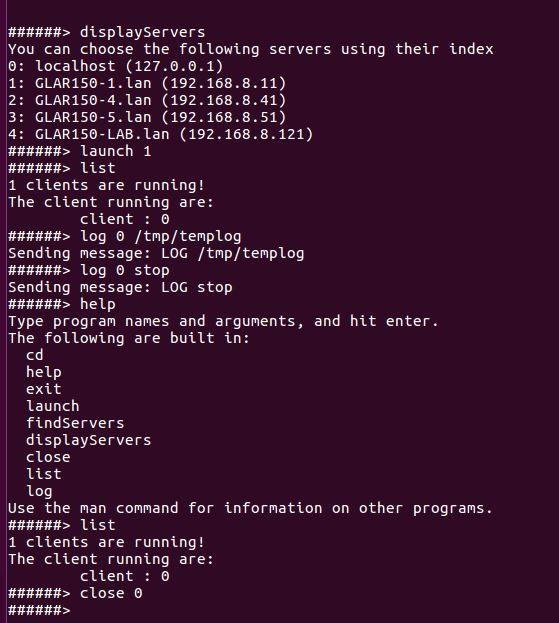
\includegraphics[width=0.7\textwidth]{image/clientshell.jpg}%
\caption{Using the client\_shell}%
\label{figure:clientshell}%-
\end{center}
\end{figure}

On the above figure, we can see how to use the client\_shell with an example.
I am launching a client for the server 1. I am telling to log the data in a file called /tmp/templog. After waiting a moment, I asked it to stop logging. At the end of the session, I am telling the client to stop the communication.


When using the launch command, a new terminal will open. This terminal is the client. It will connect to the server, print data and listen for orders from the user.

\begin{figure}[H]
\begin{center}
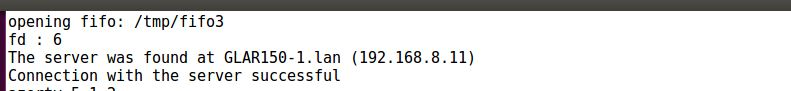
\includegraphics[width=0.7\textwidth]{image/clientinit.jpg}%
\caption{The client is connection to the server}%
\label{figure:clientint}%-
\end{center}

\end{figure}\begin{figure}[H]
\begin{center}
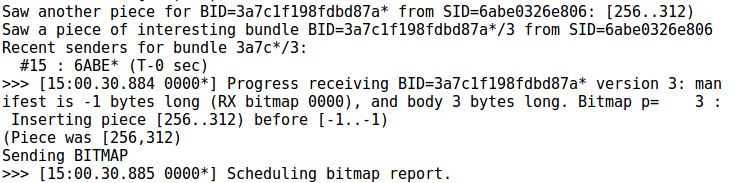
\includegraphics[width=0.7\textwidth]{image/clientcomm.jpg}%
\caption{The client is receiving data}%
\label{figure:clientcomm}%-
\end{center}

\end{figure}\begin{figure}[H]
\begin{center}
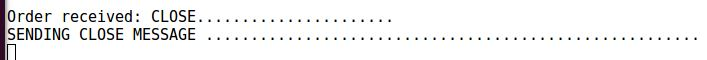
\includegraphics[width=0.7\textwidth]{image/closeclient.jpg}%
\caption{Closing the client}%
\label{figure:closeclient}%-
\end{center}
\end{figure}

The three figures above present the 3 types of action the client is executing. On the first figure, the client check if the server exists and establishes the communication with the server. On the second figure, the client is printing data received from the server. On the last figure, the client received the order "STOP" from the client\_shell (command close) and tell the server to stop before closing itself.

All these tests were made using a mockup version of the network. The server was in the same room as the computer. However, the computer had to go through the main router to reach the server. 




\section{Monitoring the Wi-Fi}

Using the workaround solution, I was able to monitor the remote router. 

\begin{figure}[H]
\begin{center}
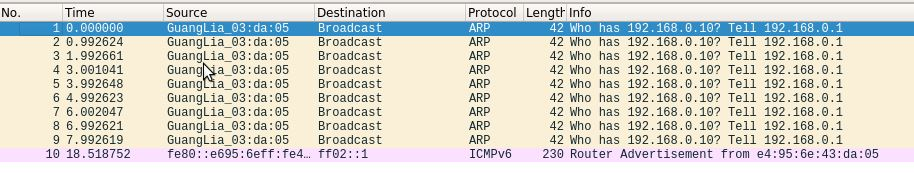
\includegraphics[width=\textwidth]{image/wireshark.jpg}%
\caption{Remote Wi-Fi analysis}%
\label{figure:wireshark}%-
\end{center}
\end{figure}

The figures show the wireshark running on the computer. The packets shown on the wireshark are packets on the LAN interface of the remote router.



\section{Remotely controlling the phone}

Currently, the remote phone control solution is not working with the small routers. As a proof of concept, it is working on a computer.
Here is the result I have using scrcpy:
\begin{figure}[H]
\begin{center}
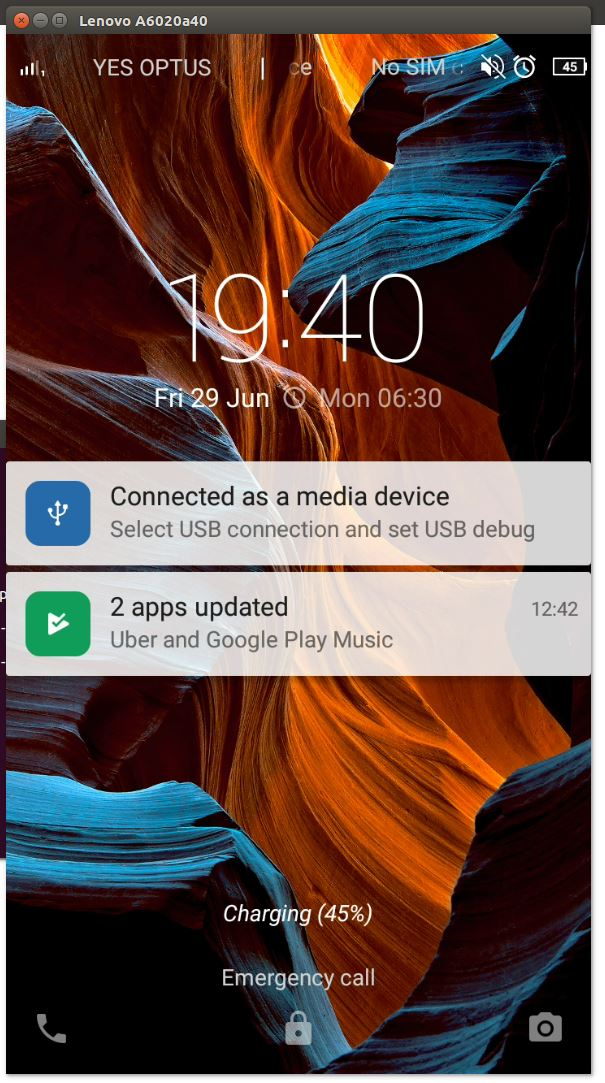
\includegraphics[width=0.3\textwidth]{image/phonecapture.jpg}%
\caption{Remote phone control}%
\label{figure:phone}%-
\end{center}
\end{figure}

On the computer, I was able to display the screen of my phone and access to everything on it. I had a full access to the phone. I could send sms or use applications from my computer.
%%%%%%%%%%%%%%%%%%%%%%%%%%%%%%%%%%%%%%%%%%%%%%%%%%%%%%%%%%%%%


\chapter{Future work}

There are some work that needs to be done to complete the solution.
First, the test network should be done in real scale in Tonsley to see if it still work in the real case.

Then, the missing features should be developed and added. 
At this point we will have a real test network.

After that, improvements can be done to the solution. For instance, I think some part of the installation process could be made easier.
Another major improvement could be to replace the client\_shell by a graphical interface. A graphical interface will make the solution more instinctive to use. That was one of my wish when I started this project. I wanted to have a graphical interface for the user. However, I knew I would not have the time to create it. That's why I decided to opt for the shell-like solution.


\chapter{Conclusion}

Overall, I am satisfied with what I was able to do in less than 2 months. I have developed a first prototype with the core features.
I think that the solution is easy to use even for someone not very familiar with the Serval project and Linux. Obviously, the user still need to know some basic about Linux and networking to install the solution. But I think that most person working on the Serval project will have some knowledge on that field and should therefore have no problem to install and use the test network. To help future users, I wrote a detailed documentation for the installation and the first use.

This project taught me a lot. I already have some knowledge on c coding, networking and Linux but I haven't trained these skills in more than a year. This project gave me some experience in this field and helped me improve. Through this project and my time spent in Australia, I have improved my English. For me it is the first time I am writing a report of this size in English. Furthermore, all the interaction with the team have made me more confident in my English skills.
 
Some mistakes were made during this project. The main mistake was the management of the different task. I feel I have lost more time than I should have on the mobile part. It was not one of the priority of the test network and I spent a lot of time on it. I could have used this time to implement the Wi-Fi part and have a better final result. I should have asked more for the help of my supervisor. I did ask some questions from time to time and his answers were really useful. But I feel like I should have asked more question and keep a better communication with my supervisor.

The project still lacks some features to be considered complete. They should be added in the future.
First, the test network should be done in real scale in Tonsley to see if it still works in the real case.

Then, the missing features should be developed and added. 
At this point we will have a real test network.

After that, improvements can be done to the solution. For instance, I think some part of the installation process could be made easier.
Another major improvement could be to replace the client\_shell by a graphical interface. A graphical interface will make the solution more instinctive to use. That was one of my wish when I started this project. I wanted to have a graphical interface for the user. However, I knew I would not have the time to create it. That's why I decided to opt for the shell-like solution.

Even if I made some mistakes and the test network is not complete yet, I am still very happy with the final result and everything I have learned.




%%%%%%%%%%%%%%%%%%%%%%%%%%%%%%%%%%%%%%%%%%%%%%%%%%%%%%%%%%%%%
%% BIBLIOGRAPHY AND OTHER LISTS
%%%%%%%%%%%%%%%%%%%%%%%%%%%%%%%%%%%%%%%%%%%%%%%%%%%%%%%%%%%%%
%% A small distance to the other stuff in the table of contents (toc)
\addtocontents{toc}{\protect\vspace*{\baselineskip}}

%% The Bibliography
%% ==> You need a file 'literature.bib' for this.
%% ==> You need to run BibTeX for this (Project | Properties... | Uses BibTeX)
%\addcontentsline{toc}{chapter}{Bibliography} %'Bibliography' into toc
%\nocite{*} %Even non-cited BibTeX-Entries will be shown.
%\bibliographystyle{alpha} %Style of Bibliography: plain / apalike / amsalpha / ...
%\bibliography{literature} %You need a file 'literature.bib' for this.

\chapter{References}

Gardner-Stephen, P., Challans, R., Lakeman, J., Bettison, A., Lieser, P., Steinmetz, R., Alvarez, F. and Lloyd, M. (2017). Productizing humanitarian telecommunications research: A case study of the Serval Mesh Extender. 2017 IEEE Global Humanitarian Technology Conference (GHTC).

\hfill \break
Gardner-Stephen, P., Farouque, S., Lloyd, M., Bate, A. and Cullen, A. (2017). Piloting the serval mesh and serval mesh extender 2.0 in Vanuatu: Preliminary results. 2017 IEEE Global Humanitarian Technology Conference (GHTC).

\hfill \break
Gardner-Stephen, P. (2018). Building an indoor test network and testing LBARD bug fixes. [online] Servalpaul.blogspot.com. Available at: \url{http://servalpaul.blogspot.com/2018/04/building-indoor-test-network-and.html} [Accessed 30 Jun. 2018].

\hfill \break
Gardner-Stephen, P. (2018). Fixing bugs and structure of LBARD. [online] Servalpaul.blogspot.com. Available at: 
\url{http://servalpaul.blogspot.com/2018/04/fixing-bugs-and-structure-of-lbard.html} [Accessed 30 Jun. 2018].

\hfill \break
Brodkin, J. (2017). Tropical Storm Harvey takes out 911 centers, cell towers, and cable networks. [online]
Ars Technica. Available at: \url{https://arstechnica.com/information-technology/2017/08/tropical-storm-harvey-
takes-out-911-centers-cell-towers-and-cable-networks/} [Accessed 15 Mar. 2018].

\hfill \break
Encyclopedia Britannica. (2017). Haiti earthquake of 2010 $|$ Effects, Damage, Map, \& Facts. [online]
Available at: \url{https://www.britannica.com/event/Haiti-earthquake-of-2010} [Accessed 15 Mar. 2018].


\hfill \break
London.gov.uk. (2007). [online] Available at:
\url{https://www.london.gov.uk/sites/default/files/gla_migrate_files_destination/archives/assembly-reports-
7july-follow-up-report.pdf} [Accessed 15 Mar. 2018].

\hfill \break
Telstra.com.au. (2018). Telstra - Our Coverage. [online] Available at: \url{https://www.telstra.com.au/coverage-
networks/our-coverage#disclaimer} [Accessed 15 Mar. 2018].


\hfill \break
Gardner-Stephen, P., Challans, R., Lakeman, J., Bettison, A., Gardner-Stephen, D. and Lloyd, M. (2013). The serval
mesh: A platform for resilient communications in disaster \&amp; crisis. 2013 IEEE Global Humanitarian Technology
Conference (GHTC).



%%%%%%%%%%%%%%%%%%%%%%%%%%%%%%%%%%%%%%%%%%%%%%%%%%%%%%%%%%%%%
%% APPENDICES
%%%%%%%%%%%%%%%%%%%%%%%%%%%%%%%%%%%%%%%%%%%%%%%%%%%%%%%%%%%%%
\appendix
%% ==> Write your text here or include other files.

%\input{FileName} %You need a file 'FileName.tex' for this.


\end{document}

